\section{伯德图绘制}

\subsection{伯德图的定义}
伯德图(Bode Plot)是由亨德里克·韦德·伯德(Hendrik Wade Bode)提出的频率响应图示方法,由两个图组成:

\begin{minipage}[t]{0.55\textwidth}
\begin{itemize}
    \item \textbf{幅频特性图(Magnitude Plot)}:$L(\omega) = 20\lg|G(\jw)|$ dB vs $\lg\omega$
    \begin{itemize}
        \item 纵轴:对数幅值(dB)
        \item 横轴:对数频率($\lg\omega$)
    \end{itemize}
    \item \textbf{相频特性图(Phase Plot)}:$\phi(\omega) = \angle G(\jw)$ vs $\lg\omega$
    \begin{itemize}
        \item 纵轴:相位角(度或弧度)
        \item 横轴:对数频率($\lg\omega$)
    \end{itemize}
\end{itemize}

\textbf{伯德图的优点:}
\begin{enumerate}
    \item 频率范围广,可表示从极低频到极高频的特性
    \item 不同环节的伯德图可以直接相加(叠加原理)
    \item 可用渐近线逼近,绘制简便
    \item 便于分析系统的稳定性和性能指标
\end{enumerate}
\end{minipage}\hfill
\begin{minipage}[t]{0.42\textwidth}
\vspace{0pt}
\textbf{典型伯德图示例:}

% 示例:一阶惯性环节 G(s) = 1/(1+0.1s)
\begin{center}
\small
\BodeTF{num/{1},den/{0.1,1}}{0.1}{1000}
\end{center}
\vspace{-0.3cm}
\begin{center}
\small
\textit{图示:$G(s) = \frac{1}{1+0.1s}$ 的伯德图}
\end{center}
\end{minipage}

\subsection{伯德图的基本概念}

伯德图由两个图组成,横坐标都是对数刻度的频率 $\omega$:
\begin{itemize}
    \item \textbf{对数幅频图}:纵坐标是系统幅值的对数 $L(\omega) = 20\log_{10}A(\omega)$,单位为分贝(dB)
    \item \textbf{对数相频图}:纵坐标是系统相角 $\phi(\omega)$,单位为度(°)
\end{itemize}

\subsubsection{对数幅频图的转折频率}

\textbf{转折频率}(Corner Frequency / Break Frequency)是渐近线斜率发生变化的频率点。

\begin{minipage}[t]{0.48\textwidth}
\begin{center}
\begin{tabular}{|c|c|c|}
\hline
\textbf{典型环节} & \textbf{传递函数} & \textbf{转折频率与斜率} \\
\hline
\multirow{2}{*}{一阶环节} & $\displaystyle\frac{1}{Ts+1}$ & $\omega_c = \frac{1}{T}$ \\ 
& & 斜率 $-20$ dB/dec \\
\hline
& $Ts+1$ & $\omega_c = \frac{1}{T}$ \\
& & 斜率 $+20$ dB/dec \\
\hline
\multirow{2}{*}{二阶环节} & $\displaystyle\frac{1}{(s/\omega_n)^2+...}$ & $\omega_c = \omega_n$ \\
& & 斜率 $-40$ dB/dec \\
\hline
& $(s/\omega_n)^2+...$ & $\omega_c = \omega_n$ \\
& & 斜率 $+40$ dB/dec \\
\hline
\end{tabular}
\end{center}
\end{minipage}\hfill
\begin{minipage}[t]{0.48\textwidth}
\vspace{0pt}
\begin{center}
\textbf{转折频率图示:}

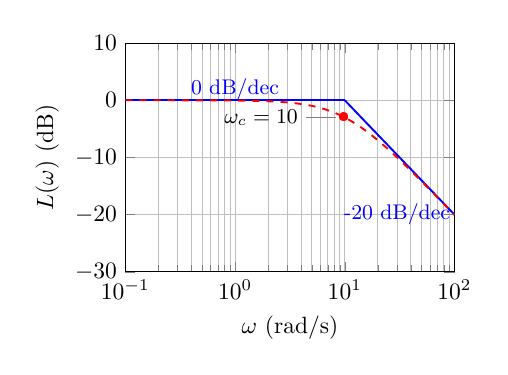
\begin{tikzpicture}[scale=0.85]
\begin{axis}[
    width=6.5cm, height=5cm,
    xmode=log,
    xlabel={$\omega$ (rad/s)},
    ylabel={$L(\omega)$ (dB)},
    grid=both,
    xmin=0.1, xmax=100,
    ymin=-30, ymax=10,
    xtick={0.1,1,10,100},
    ytick={-30,-20,-10,0,10},
]
% 渐近线
\addplot[blue, thick, domain=0.1:10] {0};
\addplot[blue, thick, domain=10:100] {-20*(log10(x)-1)};
% 精确曲线
\addplot[red, dashed, thick, samples=100, domain=0.1:100] 
    {-20*log10(sqrt(1+(x/10)^2))};
% 标注
\node[blue] at (axis cs:1,2) {\small 0 dB/dec};
\node[blue] at (axis cs:30,-20) {\small -20 dB/dec};
\node[red] at (axis cs:10,-3) [pin={180:{\small $\omega_c=10$}}] {};
\node[red] at (axis cs:10,-3) {\textbullet};
\end{axis}
\end{tikzpicture}

\small\textit{一阶极点 $G(s)=\frac{1}{1+0.1s}$ 的转折频率}
\end{center}
\end{minipage}

\vspace{0.3cm}
\textbf{关键概念:}
\begin{itemize}
    \item \textbf{渐近线}(蓝色实线):在转折频率处改变斜率
    \item \textbf{精确曲线}(红色虚线):在转折频率处与渐近线有偏差
    \item \textbf{修正值}:一阶环节在 $\omega_c$ 处偏差 $-3$ dB,二阶环节偏差 $\pm 6$ dB
\end{itemize}

\subsubsection{低频段渐近线的确定}

低频段渐近线是伯德图绘制的起点,由系统型别和增益唯一确定。

\begin{minipage}[t]{0.52\textwidth}
对于标准型 $G(s) = K \frac{\prod(1+T_i s)}{s^v\prod(1+T_j s)}$:
\begin{itemize}
    \item \textbf{斜率}:由系统型别 $v$(积分环节 $s^v$ 的个数)决定
    \begin{itemize}
        \item $v=0$(0型系统):斜率 $0$ dB/dec
        \item $v=1$(I型系统):斜率 $-20$ dB/dec
        \item $v=2$(II型系统):斜率 $-40$ dB/dec
    \end{itemize}
    \item \textbf{定位点1}:渐近线(或其延长线)\textbf{必过点 $(1, 20\lg K)$}
    \item \textbf{定位点2}($v \geq 1$ 时):与 0dB 线交于 $(\sqrt[v]{K}, 0)$
\end{itemize}

\vspace{0.2cm}
\textbf{例如:}$G(s) = \frac{10}{s(1+0.1s)}$
\begin{itemize}
    \item $K=10$,$v=1$(I型系统)
    \item 低频斜率:$-20$ dB/dec
    \item 定位点1:$(1, 20\lg 10) = (1, 20)$ dB
    \item 定位点2:$(\sqrt[1]{10}, 0) = (10, 0)$ dB
\end{itemize}
\end{minipage}\hfill
\begin{minipage}[t]{0.45\textwidth}
\vspace{0pt}
\begin{center}
\textbf{低频渐近线图示:}

\begin{tikzpicture}[scale=0.9]
\begin{axis}[
    width=6.5cm, height=6cm,
    xmode=log,
    xlabel={$\omega$ (rad/s)},
    ylabel={$L(\omega)$ (dB)},
    grid=both,
    xmin=0.1, xmax=100,
    ymin=-20, ymax=30,
    xtick={0.1,1,10,100},
    ytick={-20,0,20},
]
% 低频渐近线(延长线)
\addplot[blue, thick, dashed, domain=0.1:100] {20-20*log10(x)};
% 完整渐近线(包括转折后)
\addplot[red, very thick, domain=0.1:10] {20-20*log10(x)};
\addplot[red, very thick, domain=10:100] {20-20*log10(x)-20*log10(x/10)};

% 标注定位点
\node[red] at (axis cs:1,20) {\Large\textbullet};
\node[red, right] at (axis cs:1,20) {\small $(1, 20\lg K)$};
\node[red] at (axis cs:10,0) {\Large\textbullet};
\node[red, above right] at (axis cs:10,0) {\small $(\sqrt[v]{K}, 0)$};

% 标注斜率
\draw[<->, thick] (axis cs:1,20) -- (axis cs:10,0);
\node at (axis cs:3,12) {\small $-20v$ dB/dec};

% 标注转折频率
\node[green!60!black] at (axis cs:10,-15) [pin={90:\small 转折频率}] {};
\end{axis}
\end{tikzpicture}

\small\textit{$G(s)=\frac{10}{s(1+0.1s)}$ 的低频渐近线}
\end{center}
\end{minipage}

\subsubsection{例题:伯德图绘制示例}

\textbf{例1:绘制 $G(s) = \frac{2}{(2s+1)(8s+1)}$ 的开环对数幅频特性曲线。}

\textit{解:}
\begin{enumerate}
    \item \textbf{标准型}:$G(s) = \frac{2}{(2s+1)(8s+1)}$。开环增益 $K=2$,系统为0型 ($v=0$)
    
    \item \textbf{转折频率}:
    \begin{align*}
    T_1=2 &\implies \omega_1=\frac{1}{2}=0.5 \text{ rad/s} \\
    T_2=8 &\implies \omega_2=\frac{1}{8}=0.125 \text{ rad/s}
    \end{align*}
    按从小到大排列:$\omega_1 = 0.125$ rad/s,$\omega_2 = 0.5$ rad/s
    
    \item \textbf{低频段} ($\omega < 0.125$):
    \begin{itemize}
        \item 斜率为 $-20 \times 0 = 0$ dB/dec(水平线)
        \item 幅值为 $L(\omega) = 20\lg(2) \approx 6$ dB
    \end{itemize}
    
    \item \textbf{中频段1} ($0.125 < \omega < 0.5$):
    \begin{itemize}
        \item 经过第一个转折频率 $\omega_1 = 0.125$(一阶极点)
        \item 斜率变为 $0 - 20 = -20$ dB/dec
    \end{itemize}
    
    \item \textbf{高频段} ($\omega > 0.5$):
    \begin{itemize}
        \item 经过第二个转折频率 $\omega_2 = 0.5$(一阶极点)
        \item 斜率变为 $-20 - 20 = -40$ dB/dec
    \end{itemize}
\end{enumerate}

\subsection{典型环节的伯德图}

\subsubsection{比例环节 \texorpdfstring{$K$}{K}}
传递函数:$G(s) = K$

频率响应:$G(\jw) = K$

\textbf{幅频特性:}
\begin{align*}
L(\omega) &= 20\lg K \text{ dB(水平线)}
\end{align*}

\textbf{相频特性:}
\begin{align*}
\phi(\omega) &= \begin{cases}
0° & K > 0 \\
180° & K < 0
\end{cases}
\end{align*}

\textbf{伯德图示例:}$G(s) = 2$
\begin{center}
\BodeTF{num/{2},den/{1}}{0.1}{1000}
\end{center}

\subsubsection{积分环节 $\frac{1}{s}$}
传递函数:$G(s) = \frac{1}{s}$

频率响应:$G(\jw) = \frac{1}{\jw}$

\textbf{幅频特性:}
\begin{align*}
L(\omega) &= 20\lg\frac{1}{\omega} = -20\lg\omega \text{ dB}
\end{align*}
\begin{itemize}
    \item 斜率:$-20$ dB/十倍频(decade)
    \item 当 $\omega = 1$ rad/s 时,$L(\omega) = 0$ dB
    \item 当 $\omega$ 增大10倍时,$L(\omega)$ 下降20 dB
\end{itemize}

\textbf{相频特性:}
\begin{align*}
\phi(\omega) &= -90°\text{(恒定)}
\end{align*}

\textbf{伯德图示例:}$G(s) = \frac{1}{s}$
\begin{center}
\BodeTF{num/{1},den/{1,0}}{0.1}{1000}
\end{center}

\subsubsection{微分环节 $s$}
与积分环节对称:
\begin{itemize}
    \item $L(\omega) = 20\lg\omega$ dB(斜率 $+20$ dB/十倍频)
    \item $\phi(\omega) = 90°$
\end{itemize}

\textbf{伯德图示例:}$G(s) = s$
\begin{center}
\BodeTF{num/{1,0},den/{1}}{0.1}{1000}
\end{center}

\subsubsection{惯性环节 \texorpdfstring{$\frac{1}{1+Ts}$}{1/(1+Ts)}}
传递函数:$G(s) = \frac{1}{1+Ts}$

频率响应:$G(\jw) = \frac{1}{1+\jw T}$

\textbf{转折频率(Corner Frequency):}$\omega_c = \frac{1}{T}$ rad/s

\textbf{幅频特性:}
\begin{align*}
L(\omega) &= 20\lg|G(\jw)| = -20\lg\sqrt{1 + \omega^2T^2}
\end{align*}

渐近线:
\begin{itemize}
    \item 当 $\omega \ll \omega_c$:$L(\omega) \approx 0$ dB
    \item 当 $\omega \gg \omega_c$:$L(\omega) \approx -20\lg(\omega T)$ dB(斜率 $-20$ dB/十倍频)
    \item 转折点 $\omega = \omega_c$:精确值 $L(\omega_c) = -3$ dB
\end{itemize}

\textbf{相频特性:}
\begin{align*}
\phi(\omega) &= -\arctan(\omega T)
\end{align*}
\begin{itemize}
    \item $\omega = 0.1\omega_c$:$\phi \approx -6°$
    \item $\omega = \omega_c$:$\phi = -45°$
    \item $\omega = 10\omega_c$:$\phi \approx -84°$
    \item $\omega \to \infty$:$\phi \to -90°$
\end{itemize}

\textbf{伯德图示例:}$G(s) = \frac{1}{1+0.1s}$ ($\omega_c = 10$ rad/s)
\begin{center}
\BodeTF{num/{1},den/{0.1,1}}{0.1}{1000}
\end{center}

\subsubsection{一阶微分环节 $1+Ts$}
与惯性环节对称:
\begin{itemize}
    \item 幅频特性:低频0 dB,高频斜率 $+20$ dB/十倍频
    \item 相频特性:$\phi(\omega) = \arctan(\omega T)$,$\phi(\omega_c) = 45°$
\end{itemize}

\textbf{伯德图示例:}$G(s) = 1 + 0.1s$ ($\omega_c = 10$ rad/s)
\begin{center}
\BodeTF{num/{0.1,1},den/{1}}{0.1}{1000}
\end{center}

\subsubsection{振荡环节 $\frac{\omega_n^2}{s^2 + 2\zeta\omega_n s + \omega_n^2}$}
传递函数标准形式:
\begin{align*}
G(s) = \frac{\omega_n^2}{s^2 + 2\zeta\omega_n s + \omega_n^2}
\end{align*}

其中:
\begin{itemize}
    \item $\omega_n$:无阻尼自然频率
    \item $\zeta$:阻尼比($0 < \zeta < 1$)
\end{itemize}

频率响应:
\begin{align*}
G(\jw) = \frac{\omega_n^2}{\omega_n^2 - \omega^2 + 2\jw\zeta\omega_n}
\end{align*}

\textbf{幅频特性:}
\begin{align*}
L(\omega) &= 20\lg\frac{\omega_n^2}{\sqrt{(\omega_n^2-\omega^2)^2 + (2\zeta\omega_n\omega)^2}}
\end{align*}

渐近线:
\begin{itemize}
    \item 当 $\omega \ll \omega_n$:$L(\omega) \approx 0$ dB
    \item 当 $\omega \gg \omega_n$:$L(\omega) \approx -40\lg(\omega/\omega_n)$ dB(斜率 $-40$ dB/十倍频)
    \item 转折频率:$\omega_c = \omega_n$
\end{itemize}

\textbf{谐振峰值(仅当 $\zeta < 0.707$ 时):}
\begin{itemize}
    \item 谐振频率:$\omega_r = \omega_n\sqrt{1-2\zeta^2}$
    \item 谐振峰值:$M_r = \frac{1}{2\zeta\sqrt{1-\zeta^2}}$
    \item 当 $\zeta$ 很小时,谐振峰值很大
\end{itemize}

\textbf{转折频率处的精确值:}
\begin{itemize}
    \item $L(\omega_n) = -20\lg(2\zeta)$ dB
    \item 当 $\zeta = 0.707$ 时,$L(\omega_n) = -3$ dB(无谐振)
    \item 当 $\zeta < 0.707$ 时,$L(\omega_n) > -3$ dB(有谐振)
    \item 当 $\zeta > 0.707$ 时,$L(\omega_n) < -3$ dB(过阻尼)
\end{itemize}

\textbf{相频特性:}
\begin{align*}
\phi(\omega) &= -\arctan\frac{2\zeta\omega_n\omega}{\omega_n^2-\omega^2}
\end{align*}
\begin{itemize}
    \item $\omega = \omega_n$:$\phi = -90°$(与 $\zeta$ 无关)
    \item $\omega \to 0$:$\phi \to 0°$
    \item $\omega \to \infty$:$\phi \to -180°$
    \item $\zeta$ 越小,相位变化越快
\end{itemize}

\textbf{不同阻尼比的伯德图对比:}

\begin{center}
\begin{tikzpicture}
\begin{groupplot}[
    group style={group size=1 by 2, vertical sep=0.5cm},
    width=12cm, height=4cm,
    xmode=log,
    grid=both,
    xlabel={频率 $\omega$ (rad/s)},
    xmin=0.1, xmax=1000
]
\nextgroupplot[ylabel={幅度 (dB)}, legend pos=south west, 
    legend style={fill=white, fill opacity=0.8, draw opacity=1, text opacity=1, font=\tiny}]
\addplot[blue, thick, samples=100, domain=0.1:1000] {20*log10(100/sqrt((100-x^2)^2 + (2*0.1*10*x)^2))};
\addlegendentry{$\zeta=0.1$}
\addplot[red, thick, samples=100, domain=0.1:1000] {20*log10(100/sqrt((100-x^2)^2 + (2*0.5*10*x)^2))};
\addlegendentry{$\zeta=0.5$}
\addplot[green!60!black, thick, samples=100, domain=0.1:1000] {20*log10(100/sqrt((100-x^2)^2 + (2*1.0*10*x)^2))};
\addlegendentry{$\zeta=1.0$}

\nextgroupplot[ylabel={相位 (度)}, legend pos=north east,
    legend style={fill=white, fill opacity=0.8, draw opacity=1, text opacity=1, font=\tiny}]
\addplot[blue, thick, samples=100, domain=0.1:1000] {deg(-atan2(2*0.1*10*x, 100-x^2))};
\addlegendentry{$\zeta=0.1$}
\addplot[red, thick, samples=100, domain=0.1:1000] {deg(-atan2(2*0.5*10*x, 100-x^2))};
\addlegendentry{$\zeta=0.5$}
\addplot[green!60!black, thick, samples=100, domain=0.1:1000] {deg(-atan2(2*1.0*10*x, 100-x^2))};
\addlegendentry{$\zeta=1.0$}
\end{groupplot}
\end{tikzpicture}
\end{center}

图中所有曲线对应 $\omega_n = 10$ rad/s,不同阻尼比 $\zeta$。

\textbf{伯德图示例(欠阻尼,有谐振):}$G(s) = \frac{100}{s^2 + 2s + 100}$ ($\omega_n = 10$ rad/s,$\zeta = 0.1$)
\begin{center}
\BodeTF{num/{100},den/{1,2,100}}{0.1}{1000}
\end{center}

\textbf{伯德图示例(临界阻尼):}$G(s) = \frac{100}{s^2 + 14.14s + 100}$ ($\omega_n = 10$ rad/s,$\zeta = 0.707$)
\begin{center}
\BodeTF{num/{100},den/{1,14.14,100}}{0.1}{1000}
\end{center}

\textbf{伯德图示例(过阻尼):}$G(s) = \frac{100}{s^2 + 20s + 100}$ ($\omega_n = 10$ rad/s,$\zeta = 1.0$)
\begin{center}
\BodeTF{num/{100},den/{1,20,100}}{0.1}{1000}
\end{center}

\subsection{伯德图的绘制方法}

\subsubsection{幅值近似原则(关键技巧)}

在手绘伯德图和计算剪切频率时,使用的是近似幅值而非精确值。这是加快计算的关键:

\textbf{一阶环节 $(Ts+1)$ 的近似}:
\begin{itemize}
    \item 在转折频率前($\omega < 1/T$):虚部 $T\omega < 1$,\textbf{保留常数项1}。环节幅值近似为 $1$
    \item 在转折频率后($\omega > 1/T$):虚部 $T\omega > 1$,\textbf{保留虚部项 $T\omega$}。环节幅值近似为 $T\omega$
\end{itemize}

\textbf{二阶环节 $((s/\omega_n)^2 + ...)$ 的近似}:
\begin{itemize}
    \item 在转折频率前($\omega < \omega_n$):\textbf{保留常数项1}。环节幅值近似为 $1$
    \item 在转折频率后($\omega > \omega_n$):\textbf{保留平方项 $(s/\omega_n)^2$}。环节幅值近似为 $(\omega/\omega_n)^2$
\end{itemize}

\subsubsection{伯德图绘制六步法}

这是一套标准化、模板化的绘制流程,特别适合考试手绘:

\textbf{第一步:化为"尾1"标准型}

将传递函数中所有的一阶和二阶环节都化为 $(Ts+1)$ 或 $((s/\omega_n)^2 + 2\zeta(s/\omega_n) + 1)$ 的形式。这样可以方便地读出开环增益 $K$ 和各转折频率。

标准形式为:
\begin{align*}
G(s) = K \frac{\prod(1+T_{zi}s)\prod((s/\omega_{ni})^2+2\zeta_i(s/\omega_{ni})+1)}{s^v\prod(1+T_{pi}s)\prod((s/\omega_{nj})^2+2\zeta_j(s/\omega_{nj})+1)}
\end{align*}

\textbf{第二步:列出系统的转折频率}

转折频率(交接频率)是渐近线斜率发生改变的点:
\begin{itemize}
    \item 一阶环节 $(Ts \pm 1)$:转折频率为 $\omega_c = \frac{1}{T}$
    \item 二阶环节 $((s/\omega_n)^2 + ...)$:转折频率为 $\omega_c = \omega_n$
\end{itemize}

\textbf{将所有转折频率从小到大排列}。

\textbf{第三步:确定开环增益 $K$}

从"尾1"标准型中直接读出比例项 $K$。

\textbf{第四步:求与横轴的交点(剪切频率 $\omega_{gc}$)}

横轴(0dB 线)代表 $|G(j\omega)| = 1$。需要求解方程 $|G(j\omega_{gc})| = 1$,利用下面的"幅值近似原则"。

\textbf{第五步:绘制低频段渐近线}

低频段渐近线由以下三个性质唯一确定:
\begin{enumerate}
    \item \textbf{斜率}:由系统型别 $v$(积分环节 $s^v$ 的个数)决定,斜率为 $-20v$ dB/dec
    \item \textbf{定位点1}:低频段渐近线(或其延长线)\textbf{必过点 $(\omega=1, 20\log_{10}K)$}
    \item \textbf{定位点2($v \geq 1$ 时)}:低频段渐近线(或其延长线)\textbf{与0dB横轴相交于点 $(\omega = \sqrt[v]{K}, 0\text{ dB})$}
\end{enumerate}

\textbf{第六步:依次绘制后续曲线}

从最低的转折频率开始,每经过一个转折频率,渐近线的斜率发生一次改变:

\begin{center}
\begin{tabular}{|c|c|c|}
\hline
\textbf{典型环节} & \textbf{位置} & \textbf{斜率变化} \\
\hline
\multirow{2}{*}{一阶环节} & 分母 & $-20$ dB/dec \\
\cline{2-3}
& 分子 & $+20$ dB/dec \\
\hline
\multirow{2}{*}{二阶环节} & 分母 & $-40$ dB/dec \\
\cline{2-3}
& 分子 & $+40$ dB/dec \\
\hline
\end{tabular}
\end{center}

\textbf{【最终验证】}:绘制完成后,检查最后一个频段的斜率是否等于 $-20(n-m)$ dB/dec,其中 $n$ 是分母阶次,$m$ 是分子阶次。

\vspace{0.3cm}
\begin{tcolorbox}[colback=green!5!white,colframe=green!60!black,title=六步法绘制流程图示]
\begin{center}
\begin{tikzpicture}[scale=0.95]
\begin{axis}[
    width=13cm, height=7cm,
    xmode=log,
    xlabel={\large $\omega$ (rad/s)},
    ylabel={\large $L(\omega)$ (dB)},
    grid=both,
    xmin=0.01, xmax=100,
    ymin=-60, ymax=40,
    xtick={0.01,0.1,1,10,100},
    ytick={-60,-40,-20,0,20,40},
    legend pos=south west,
    legend style={fill=white, fill opacity=0.8, draw opacity=1, text opacity=1, font=\small},
]
% 示例系统:G(s) = 10(s+1) / [s(s+10)(s+100)]
% K=10, v=1, 转折频率: 1, 10, 100

% 低频段 (v=1, 斜率-20dB/dec)
\addplot[blue, ultra thick, domain=0.01:1] {20-20*log10(x)};
\addlegendentry{低频段:$-20$ dB/dec}

% 中频段1 (经过ω=1零点,斜率变为0)
\addplot[red, ultra thick, domain=1:10] {0};
\addlegendentry{经过零点:0 dB/dec}

% 中频段2 (经过ω=10极点,斜率变为-20)
\addplot[green!60!black, ultra thick, domain=10:100] {-20*log10(x/10)};
\addlegendentry{经过极点:$-20$ dB/dec}

% 标注关键点
\node[blue] at (axis cs:1,20) {\Large\textbullet};
\node[blue, above] at (axis cs:1,20) {\small 步骤5: $(1, 20\lg K)$};

\node[red] at (axis cs:1,0) {\Large\textbullet};
\node[red, below right] at (axis cs:1,0) {\small 步骤2: $\omega_1=1$ (零点)};

\node[green!60!black] at (axis cs:10,0) {\Large\textbullet};
\node[green!60!black, below] at (axis cs:10,0) {\small 步骤6: $\omega_2=10$ (极点)};

% 标注斜率
\draw[<->, thick, blue] (axis cs:0.1,40) -- (axis cs:1,20);
\node[blue] at (axis cs:0.3,32) {\small $-20v$};

\draw[<->, thick, red] (axis cs:2,0) -- (axis cs:8,0);
\node[red] at (axis cs:4,3) {\small $0$};

\draw[<->, thick, green!60!black] (axis cs:20,-6) -- (axis cs:80,-18);
\node[green!60!black] at (axis cs:40,-10) {\small $-20$};

\end{axis}
\end{tikzpicture}
\end{center}
\vspace{-0.2cm}
\small
\textbf{示例:}$G(s) = \frac{10(s+1)}{s(s+10)}$ 的绘制过程:
\textbf{步骤1-3:} $K=10, v=1$;\textbf{步骤2:} $\omega_1=1$ (零点), $\omega_2=10$ (极点);
\textbf{步骤5:} 从 $(1,20)$ dB 开始,斜率 $-20$ dB/dec;
\textbf{步骤6:} 在 $\omega_1=1$ 处斜率 $+20$,变为 0 dB/dec;在 $\omega_2=10$ 处斜率 $-20$,变为 $-20$ dB/dec
\end{tcolorbox}

\subsubsection{转折频率处的修正}

渐近线在转折频率附近与精确曲线存在偏差,需要修正以提高精度。

\begin{minipage}[t]{0.48\textwidth}
\textbf{一阶环节 $\frac{1}{1+Ts}$ 的修正:}

\begin{center}
\begin{tabular}{c|c|c}
\hline
频率 & 渐近线误差 & 精确值修正 \\
\hline
$0.5\omega_c$ & $0$ dB & $-1$ dB \\
$\omega_c$ & $0$ dB & $\textbf{-3 dB}$ \\
$2\omega_c$ & $0$ dB & $-1$ dB \\
\hline
\end{tabular}
\end{center}

\vspace{0.3cm}
\textbf{二阶环节的修正}

取决于阻尼比 $\zeta$,在 $\omega = \omega_n$ 处:
\begin{itemize}
    \item $\zeta = 0.1$:谐振峰值约 $+14$ dB
    \item $\zeta = 0.2$:谐振峰值约 $+7$ dB
    \item $\zeta = 0.3$:谐振峰值约 $+3$ dB
    \item $\zeta = 0.5$:误差约 $-1$ dB
    \item $\zeta = 0.707$:误差 $\textbf{-3 dB}$(临界阻尼)
    \item $\zeta = 1.0$:误差 $-6$ dB(过阻尼)
\end{itemize}
\end{minipage}\hfill
\begin{minipage}[t]{0.48\textwidth}
\vspace{0pt}
\begin{center}
\textbf{修正值图示(一阶极点):}

\begin{tikzpicture}[scale=0.9]
\begin{axis}[
    width=6.5cm, height=5.5cm,
    xmode=log,
    xlabel={$\omega/\omega_c$},
    ylabel={$L(\omega)$ (dB)},
    grid=both,
    xmin=0.1, xmax=10,
    ymin=-25, ymax=5,
    xtick={0.1,0.5,1,2,10},
    xticklabels={$0.1\omega_c$,$0.5\omega_c$,$\omega_c$,$2\omega_c$,$10\omega_c$},
    ytick={-20,-10,-3,0},
    legend pos=south west,
    legend style={fill=white, fill opacity=0.8, draw opacity=1, text opacity=1, font=\tiny},
]
% 渐近线
\addplot[blue, thick, domain=0.1:1] {0};
\addplot[blue, thick, domain=1:10] {-20*(log10(x))};
\addlegendentry{渐近线}

% 精确曲线
\addplot[red, thick, dashed, samples=100, domain=0.1:10] 
    {-20*log10(sqrt(1+x^2))};
\addlegendentry{精确曲线}

% 标注修正点
\node[green!60!black] at (axis cs:0.5,-1) {\textbullet};
\node[green!60!black, left] at (axis cs:0.5,-1) {\tiny $-1$ dB};

\node[green!60!black] at (axis cs:1,-3) {\Large\textbullet};
\node[green!60!black, right] at (axis cs:1,-3) {\small $-3$ dB};

\node[green!60!black] at (axis cs:2,-7) {\textbullet};
\node[green!60!black, right] at (axis cs:2,-7) {\tiny $-1$ dB};

\end{axis}
\end{tikzpicture}

\small\textit{一阶环节的渐近线与精确曲线对比}
\end{center}
\end{minipage}

\subsubsection{六步法综合例题}

\textbf{例1:绘制 $G(s) = \frac{8(\frac{s}{0.1}+1)}{s(s^2+s+1)(\frac{s}{2}+1)}$ 的开环对数幅频特性曲线。}

\textit{解:}
\begin{enumerate}
    \item \textbf{化为标准型}:
    \[G(s) = \frac{8(10s+1)}{s(s^2+s+1)(0.5s+1)}\]
    
    \item \textbf{转折频率}:
    \begin{itemize}
        \item 分子一阶:$T_z=10 \implies \omega_1 = \frac{1}{10} = 0.1$ rad/s(零点,+20 dB/dec)
        \item 分母二阶:由 $s^2+s+1 = 0$ 得 $2\zeta\omega_n = 1, \omega_n^2 = 1$,所以 $\omega_n=1$ rad/s(极点,-40 dB/dec)
        \item 分母一阶:$T_p=0.5 \implies \omega_3 = \frac{1}{0.5} = 2$ rad/s(极点,-20 dB/dec)
        \item 排序:$0.1, 1, 2$
    \end{itemize}
    
    \item \textbf{开环增益}:$K = 8$
    
    \item \textbf{低频段} ($\omega < 0.1$):
    \begin{itemize}
        \item 系统为I型 ($v=1$),斜率为 $-20$ dB/dec
        \item 与0dB轴交于 $\omega = \sqrt[1]{K} = 8$ rad/s
        \item 但 $8 > 0.1$,说明交点不在低频段
        \item 可用定位点:在 $\omega=1$ 处,幅值为 $L(1) = 20\lg 8 - 20 \times 1 = 18.06$ dB
    \end{itemize}
    
    \item \textbf{各频段渐近线}:
    \begin{itemize}
        \item $0.1 < \omega < 1$:经过 $\omega_1=0.1$(分子一阶零点),斜率变为 $-20+20=0$ dB/dec
        \item $1 < \omega < 2$:经过 $\omega_2=1$(分母二阶极点),斜率变为 $0-40=-40$ dB/dec
        \item $\omega > 2$:经过 $\omega_3=2$(分母一阶极点),斜率变为 $-40-20=-60$ dB/dec
    \end{itemize}
    
    \item \textbf{最终验证}:
    \begin{itemize}
        \item 分子阶次 $m=1$(一阶零点)
        \item 分母阶次 $n=4$(1个一阶 + 1个二阶 + 1个积分 = 4)
        \item 最终斜率应为 $-20(n-m) = -20(4-1) = -60$ dB/dec,正确✓
    \end{itemize}
\end{enumerate}

\subsubsection{剪切频率的计算}

剪切频率(增益穿越频率 $\omega_{gc}$)是幅值等于1(0 dB)的频率,通过求解 $|G(j\omega_{gc})| = 1$ 得到。

\textbf{计算方法}:利用幅值近似原则
\begin{enumerate}
    \item 在不同频段,根据主导环节使用近似幅值
    \item 在所有转折频率处分别计算幅值,判断穿越点在哪一段
    \item 在该频段内使用简化的近似幅值公式求解
\end{enumerate}

\textbf{典型例子}:$G(s) = \frac{2}{(2s+1)(8s+1)}$

设 $\omega_1 = 0.125, \omega_2 = 0.5$,则:
\begin{itemize}
    \item 低频 $\omega < 0.125$:$|G(j\omega)| \approx 2$(>1),不包含穿越点
    \item 中频 $0.125 < \omega < 0.5$:$|G(j\omega)| \approx \frac{2}{8\omega}$
    \begin{itemize}
        \item 令 $\frac{2}{8\omega} = 1 \implies \omega = 0.25$
        \item 由于 $0.125 < 0.25 < 0.5$,假设成立,所以 $\omega_{gc} = 0.25$
    \end{itemize}
    \item 高频验证:若需更精确,可用精确公式验证
\end{itemize}

\subsubsection{绘图示例}

\textbf{例1:}绘制 $G(s) = \frac{10}{s(1+0.1s)}$ 的伯德图

\begin{tcolorbox}[colback=blue!5!white,colframe=blue!75!black,title=例1求解过程与伯德图]

\begin{minipage}[t]{0.47\textwidth}
\textbf{解:}
\begin{enumerate}
    \item 标准形式:$G(s) = \frac{10}{s(1+0.1s)}$,$K = 10$
    \item 环节识别:
    \begin{itemize}
        \item 积分环节:$\frac{1}{s}$($v=1$)
        \item 惯性环节:$\frac{1}{1+0.1s}$,$T=0.1$
    \end{itemize}
    \item 转折频率:$\omega_c = \frac{1}{T} = 10$ rad/s
    \item 幅频特性:
    \begin{itemize}
        \item 起点:$L(1) = 20$ dB
        \item $\omega < 10$:$-20$ dB/十倍频
        \item $\omega > 10$:$-40$ dB/十倍频
        \item 修正:$-3$ dB @ $\omega=10$
    \end{itemize}
    \item 相频特性:
    \begin{itemize}
        \item $\phi(\omega) = -90° - \arctan(0.1\omega)$
        \item @ $\omega = 10$:$\phi = -135°$
    \end{itemize}
\end{enumerate}
\end{minipage}\hfill
\begin{minipage}[t]{0.47\textwidth}
% G(s) = 10/(s(1+0.1s)) -> num=10, den=0.1 s^2 + 1 s + 0
\BodeTF{num/{10},den/{0.1,1,0}}{0.1}{1000}
\end{minipage}

\end{tcolorbox}

\textbf{例2:}绘制 $G(s) = \frac{100(s+1)}{s(s+10)}$ 的伯德图

\begin{tcolorbox}[colback=blue!5!white,colframe=blue!75!black,title=例2求解过程与伯德图]

\begin{minipage}[t]{0.47\textwidth}
\textbf{解:}
\begin{enumerate}
    \item 标准形式:$G(s) = \frac{10(1+s)}{s(1+0.1s)}$,$K = 10$
    \item 环节识别:
    \begin{itemize}
        \item 积分环节:$\frac{1}{s}$
        \item 一阶零点:$(1+s)$
        \item $\omega_{c1} = 1$ rad/s
        \item 一阶极点:$\frac{1}{1+0.1s}$
        \item $\omega_{c2} = 10$ rad/s
    \end{itemize}
    \item 转折频率:$1$ rad/s(零点),$10$ rad/s(极点)
    \item 幅频特性:
    \begin{itemize}
        \item 低频 $\omega<1$:$-20$ dB/十倍频
        \item 中频 $1<\omega<10$:$0$ dB/十倍频
        \item 高频 $\omega>10$:$-20$ dB/十倍频
    \end{itemize}
    \item 相频特性:
    \begin{itemize}
        \item $\phi(\omega) = -90° + \arctan(\omega)$ 
        \item $\quad - \arctan(0.1\omega)$
    \end{itemize}
\end{enumerate}
\end{minipage}\hfill
\begin{minipage}[t]{0.47\textwidth}
% G(s) = 100(s+1)/(s(s+10)) -> num=100 s + 100, den = s^2 + 10 s + 0
\BodeTF{num/{100,100},den/{1,10,0}}{0.1}{1000}
\end{minipage}

\end{tcolorbox}

\textbf{例3:}二阶系统 $G(s) = \frac{100}{s^2 + 2s + 100}$

\begin{tcolorbox}[colback=blue!5!white,colframe=blue!75!black,title=例3求解过程与伯德图]

\begin{minipage}[t]{0.47\textwidth}
\textbf{解:}
\begin{enumerate}
    \item 标准形式:
    $$G(s) = \frac{\omega_n^2}{s^2 + 2\zeta\omega_n s + \omega_n^2}$$
    
    \item 参数识别:
    \begin{itemize}
        \item $\omega_n = 10$ rad/s
        \item $\zeta = 0.1$
        \item 极点:$-1 \pm 9.95j$
    \end{itemize}
    
    \item 特性分析:
    \begin{itemize}
        \item 转折频率:$10$ rad/s
        \item $\zeta < 0.707$,有谐振
        \item 谐振频率:$\approx 9.9$ rad/s
        \item 谐振峰值:$\approx 5.03$(14 dB)
    \end{itemize}
\end{enumerate}
\end{minipage}\hfill
\begin{minipage}[t]{0.47\textwidth}
\BodeTF{num/{100},den/{1,2,100}}{0.1}{1000}
\end{minipage}

\end{tcolorbox}

\subsubsection{快速参考}

以下表格是伯德图绘制中各种典型环节的\textbf{快速参考},可在考试或实际绘图时查阅。

\textbf{1. 伯德图绘制规则速查表}

{\renewcommand{\arraystretch}{2.0}
\small
\begin{center}
\begin{tabular}{|c|c|c|p{4.8cm}|c|}
\hline
\rowcolor{blue!30}
\multicolumn{5}{|c|}{\Large\textbf{伯德图典型环节速查表}} \\
\hline
\rowcolor{blue!15}
\textbf{环节} & \textbf{传递函数} & \textbf{转折频率} & \textbf{幅频斜率} & \textbf{相频} \\
\hline

\rowcolor{gray!8}
\textbf{比例} & $K$ & — & $0$ dB/dec & $0°/180°$ \\
\hline

\rowcolor{white}
\textbf{积分} & $\frac{1}{s}$ & — & $-20$ dB/dec & $-90°$ \\
\hline

\rowcolor{gray!8}
\textbf{微分} & $s$ & — & $+20$ dB/dec & $+90°$ \\
\hline

\rowcolor{white}
\textbf{一阶极点} & $\frac{1}{1+Ts}$ & $\omega_c = \frac{1}{T}$ & 
低频:$0$;高频:$-20$ dB/dec & 
$-45°$ @ $\omega_c$ \\
\hline

\rowcolor{gray!8}
\textbf{一阶零点} & $1+Ts$ & $\omega_c = \frac{1}{T}$ & 
低频:$0$;高频:$+20$ dB/dec & 
$+45°$ @ $\omega_c$ \\
\hline

\rowcolor{white}
\textbf{二阶极点} & $\frac{\omega_n^2}{(s/\omega_n)^2+2\zeta(s/\omega_n)+1}$ & $\omega_c = \omega_n$ & 
低频:$0$;高频:$-40$ dB/dec & 
$-90°$ @ $\omega_n$ \\
\hline

\rowcolor{gray!8}
\textbf{二阶零点} & $(s/\omega_n)^2+2\zeta(s/\omega_n)+1$ & $\omega_c = \omega_n$ & 
低频:$0$;高频:$+40$ dB/dec & 
$+90°$ @ $\omega_n$ \\
\hline

\end{tabular}
\end{center}
}

\textbf{快速参考提示:}
\begin{itemize}
    \item \textbf{转折点修正}:一阶环节修正 $\pm 3$ dB,二阶环节修正 $\pm 6$ dB
    \item \textbf{极点}:幅频向下(负斜率),相频向下(变负)
    \item \textbf{零点}:幅频向上(正斜率),相频向上(变正)
    \item \textbf{积分/微分}:无转折频率,斜率固定
\end{itemize}

\vspace{0.3cm}
\textbf{典型环节斜率可视化对比:}

\begin{center}
\begin{tikzpicture}
\begin{axis}[
    width=14cm, height=6cm,
    xmode=log,
    xlabel={$\omega$ (rad/s)},
    ylabel={$L(\omega)$ (dB)},
    grid=both,
    xmin=0.1, xmax=100,
    ymin=-50, ymax=50,
    xtick={0.1,1,10,100},
    ytick={-40,-20,0,20,40},
    legend columns=3,
    legend style={
        at={(0.5,1.02)},
        anchor=south,
        font=\scriptsize,
        column sep=0.5cm,
        /tikz/every even column/.append style={column sep=0.3cm}
    },
]
% 积分环节 1/s (斜率-20)
\addplot[blue, ultra thick, domain=0.1:100] {20-20*log10(x)};
\addlegendentry{积分 $\frac{1}{s}$: $-20$ dB/dec}

% 比例环节 K=10
\addplot[black, thick, domain=0.1:100] {20};
\addlegendentry{比例 $K=10$: 0 dB/dec}

% 微分环节 s (斜率+20)
\addplot[green!60!black, ultra thick, domain=0.1:100] {20*log10(x)};
\addlegendentry{微分 $s$: $+20$ dB/dec}

% 一阶极点 (转折频率10)
\addplot[red, thick, dashed, domain=0.1:10] {0};
\addplot[red, thick, dashed, domain=10:100] {-20*log10(x/10)};
\addlegendentry{一阶极点 $\frac{1}{1+0.1s}$: 0→$-20$ dB/dec}

% 一阶零点 (转折频率10)
\addplot[orange, thick, dotted, domain=0.1:10] {0};
\addplot[orange, thick, dotted, domain=10:100] {20*log10(x/10)};
\addlegendentry{一阶零点 $1+0.1s$: 0→$+20$ dB/dec}

\end{axis}
\end{tikzpicture}
\end{center}

\vspace{0.3cm}
\textbf{2. 修正值详表}

极点与零点总是"互为镜像"的,掌握以下规律能加快绘图速度。

{\renewcommand{\arraystretch}{1.6}
\begin{center}
\small
\begin{tabular}{|c|c|c|}
\hline
\rowcolor{blue!20}
\textbf{特征} & \textbf{一阶/二阶极点} & \textbf{一阶/二阶零点} \\
\hline
\rowcolor{gray!5}
\textbf{斜率变化} & 负值(衰减) & 正值(增强) \\
\hline
\textbf{相位变化方向} & 向下(越来越负) & 向上(越来越正) \\
\hline
\rowcolor{gray!5}
\textbf{在转折点修正} & 减少 $\pm 3$ dB / $\pm 6$ dB & 增加 $\pm 3$ dB / $\pm 6$ dB \\
\hline
\textbf{谐振特征} & 可能出现谐振峰 & 可能出现谷值 \\
\hline
\end{tabular}
\end{center}
}

\textbf{一阶环节(极点和零点)修正值参考}

\begin{center}
\small
\begin{tabular}{|c|c|c|c|}
\hline
\textbf{环节} & \textbf{频率点} & \textbf{修正值} & \textbf{说明} \\
\hline
\multirow{3}{*}{\shortstack{一阶极点 \\ $\frac{1}{1+Ts}$}} & $0.5\omega_c$ & $-1$ dB & 稍低于渐近线 \\
\cline{2-4}
& $\omega_c$ & $-3$ dB & 精确值 \\
\cline{2-4}
& $2\omega_c$ & $-1$ dB & 稍低于渐近线 \\
\hline
\multirow{3}{*}{\shortstack{一阶零点 \\ $1+Ts$}} & $0.5\omega_c$ & $+1$ dB & 稍高于渐近线 \\
\cline{2-4}
& $\omega_c$ & $+3$ dB & 精确值 \\
\cline{2-4}
& $2\omega_c$ & $+1$ dB & 稍高于渐近线 \\
\hline
\end{tabular}
\end{center}

\textbf{二阶极点 — 不同阻尼比下的谐振特性}

\begin{center}
\small
\begin{tabular}{|c|c|c|c|}
\hline
\textbf{阻尼比 $\zeta$} & \textbf{在 $\omega=\omega_n$ 处} & \textbf{幅值(dB)} & \textbf{特征分类} \\
\hline
$0.1 \sim 0.3$ & 明显谐振峰 & $+3$ 到 $+14$ dB & 强谐振 \\
\hline
$0.5$ & 轻微谐振 & $\approx -1$ dB & 中等阻尼 \\
\hline
$0.707$ & 临界点 & $-3$ dB & \textbf{临界阻尼} \\
\hline
$1.0$ 以上 & 过阻尼 & $-6$ dB 以下 & 无谐振 \\
\hline
\end{tabular}
\end{center}

\vspace{0.3cm}
\textit{提示:当 $\zeta > 0.707$ 时,二阶极点的行为接近两个一阶极点,可用叠加法求解。}

\subsection{伯德图的应用}

\subsubsection{由伯德图确定传递函数}

根据伯德图的幅频特性,可以反推传递函数。这是伯德图绘制的逆过程。

\textbf{基本步骤:}
\begin{enumerate}
    \item \textbf{从低频渐近线确定系统型别 $v$ 和增益 $K$}
    \begin{itemize}
        \item 低频渐近线斜率 = $-20v$ dB/dec,确定积分环节数 $v$
        \item 低频渐近线(或其延长线)过点 $(1, 20\lg K)$,确定增益 $K$
    \end{itemize}
    
    \item \textbf{从转折频率确定各环节的时间常数}
    \begin{itemize}
        \item 一阶环节:$\omega_c = \frac{1}{T} \implies T = \frac{1}{\omega_c}$
        \item 二阶环节:$\omega_c = \omega_n$
    \end{itemize}
    
    \item \textbf{从斜率变化确定零极点类型}
    \begin{itemize}
        \item 斜率增加 $+20$ dB/dec:分子一阶(零点)
        \item 斜率减少 $-20$ dB/dec:分母一阶(极点)
        \item 斜率增加 $+40$ dB/dec:分子二阶(零点)
        \item 斜率减少 $-40$ dB/dec:分母二阶(极点)
    \end{itemize}
    
    \item \textbf{组合得到传递函数}
    \begin{itemize}
        \item 将所有环节相乘得到标准型传递函数
    \end{itemize}
\end{enumerate}

\textbf{例题:已知系统的伯德图如下,求其传递函数。}

\begin{minipage}[t]{0.48\textwidth}
\textbf{解题分析:}

从给定的伯德图观察:

\textbf{步骤1:确定型别和增益}
\begin{itemize}
    \item 低频段斜率:$-20$ dB/dec
    \item 系统型别:$v = 1$(I型系统)
    \item 延长低频线过点 $(1, 40)$ dB
    \item 增益:$K = 10^{40/20} = 100$
\end{itemize}

\textbf{步骤2-3:识别转折频率和环节}
\begin{itemize}
    \item $\omega_1 = 1$ rad/s:斜率从 $-20$ 变为 $0$
    \begin{itemize}
        \item 变化:$+20$ dB/dec
        \item 环节:分子一阶零点 $(1+s)$
    \end{itemize}
    \item $\omega_2 = 10$ rad/s:斜率从 $0$ 变为 $-20$
    \begin{itemize}
        \item 变化:$-20$ dB/dec
        \item 环节:分母一阶极点 $\frac{1}{1+0.1s}$
    \end{itemize}
\end{itemize}

\textbf{步骤4:组合传递函数}
\begin{align*}
G(s) &= \frac{K(1+s)}{s(1+0.1s)} \\
&= \frac{100(s+1)}{s(s+10)}
\end{align*}

\textbf{验证:}
\begin{itemize}
    \item 低频段:$L(1) = 20\lg 100 - 20 = 40$ dB ✓
    \item 转折频率:$1, 10$ rad/s ✓
    \item 最终斜率:$-20(2-1) = -20$ dB/dec ✓
\end{itemize}
\end{minipage}\hfill
\begin{minipage}[t]{0.48\textwidth}
\vspace{0pt}
\textbf{伯德图(已知):}

\begin{center}
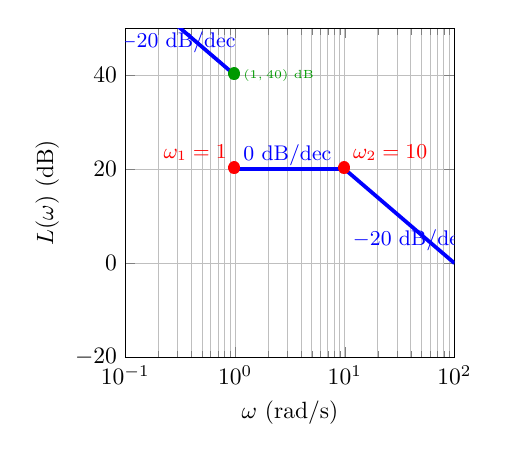
\begin{tikzpicture}[scale=0.85]
\begin{axis}[
    width=6.5cm, height=6.5cm,
    xmode=log,
    xlabel={$\omega$ (rad/s)},
    ylabel={$L(\omega)$ (dB)},
    grid=both,
    xmin=0.1, xmax=100,
    ymin=-20, ymax=50,
    xtick={0.1,1,10,100},
    ytick={-20,0,20,40},
]
% 渐近线
\addplot[blue, ultra thick, domain=0.1:1] {40-20*log10(x)};
\addplot[blue, ultra thick, domain=1:10] {20};
\addplot[blue, ultra thick, domain=10:100] {20-20*log10(x/10)};

% 标注转折频率
\node[red] at (axis cs:1,20) {\Large\textbullet};
\node[red, above left] at (axis cs:1,20) {\small $\omega_1=1$};

\node[red] at (axis cs:10,20) {\Large\textbullet};
\node[red, above right] at (axis cs:10,20) {\small $\omega_2=10$};

% 标注斜率
\node[blue] at (axis cs:0.3,47) {\small $-20$ dB/dec};
\node[blue] at (axis cs:3,23) {\small $0$ dB/dec};
\node[blue] at (axis cs:40,5) {\small $-20$ dB/dec};

% 标注定位点
\node[green!60!black] at (axis cs:1,40) {\Large\textbullet};
\node[green!60!black, right] at (axis cs:1,40) {\tiny $(1, 40)$ dB};

\end{axis}
\end{tikzpicture}
\end{center}
\end{minipage}

\vspace{0.3cm}
\textbf{关键技巧总结:}
\begin{itemize}
    \item \textbf{低频段是关键}:从低频渐近线可以确定 $K$ 和 $v$
    \item \textbf{转折频率即环节参数}:直接读出时间常数或自然频率
    \item \textbf{斜率变化即环节类型}:$\pm 20$ 是一阶,$\pm 40$ 是二阶;正号是零点,负号是极点
    \item \textbf{最终验证很重要}:检查分子分母阶次与最终斜率是否匹配
\end{itemize}

\subsubsection{稳定性分析}

伯德图可以直观地分析闭环系统的稳定性,通过增益裕度和相位裕度来量化稳定裕量。

\begin{minipage}[t]{0.52\textwidth}
\textbf{增益裕度(Gain Margin,GM):}
\begin{align*}
\text{GM} = -L(\omega_g) \text{ dB}
\end{align*}
其中 $\omega_g$ 为\textbf{相位穿越频率}($\phi(\omega_g) = -180°$)

\textbf{物理意义:}系统增益可以增加多少倍而不失稳

\vspace{0.3cm}
\textbf{相位裕度(Phase Margin,PM):}
\begin{align*}
\text{PM} = 180° + \phi(\omega_c)
\end{align*}
其中 $\omega_c$ 为\textbf{剪切频率}(增益穿越频率,$L(\omega_c) = 0$ dB)

\textbf{物理意义:}相位可以再滞后多少度而不失稳

\vspace{0.3cm}
\textbf{稳定性判据:}
\begin{itemize}
    \item \textbf{稳定条件}:GM $> 0$ dB 且 PM $> 0°$
    \item \textbf{一般要求}:GM $\geq 6$ dB,PM $\geq 30°$
    \item \textbf{良好性能}:GM $\geq 10$ dB,PM $\geq 45°$
\end{itemize}

\vspace{0.2cm}
\textbf{裕度与性能的关系:}
\begin{itemize}
    \item PM $\approx 45°$:超调量 $\sigma\% \approx 20\%$
    \item PM $\approx 60°$:超调量 $\sigma\% \approx 10\%$
    \item PM 越大,系统越稳定,但响应越慢
    \item GM 和 PM 越大,系统对参数变化越不敏感
\end{itemize}
\end{minipage}\hfill
\begin{minipage}[t]{0.45\textwidth}
\vspace{0pt}
\textbf{裕度图示:}

\begin{center}
\begin{tikzpicture}
\begin{groupplot}[
    group style={group size=1 by 2, vertical sep=0.3cm},
    width=6.5cm, height=3.5cm,
    xmode=log,
    grid=both,
    xmin=0.1, xmax=100,
]
\nextgroupplot[ylabel={$L(\omega)$ (dB)}, ytick={-20,0,20}, ymin=-25, ymax=25]
% 幅频曲线
\addplot[blue, thick, samples=100, domain=0.1:100] 
    {20-20*log10(x)-20*log10(sqrt(1+(x/10)^2))};
% 0dB线
\addplot[red, dashed] coordinates {(0.1,0) (100,0)};
% 标注
\node[red] at (axis cs:3,0) {\textbullet};
\node[red, above] at (axis cs:3,3) {\tiny $\omega_c$ (剪切频率)};
\node[green!60!black] at (axis cs:15,-10) {\textbullet};
\node[green!60!black, below] at (axis cs:15,-13) {\tiny GM};
\draw[<->, green!60!black, thick] (axis cs:15,-10) -- (axis cs:15,0);

\nextgroupplot[ylabel={$\phi(\omega)$ (°)}, xlabel={$\omega$ (rad/s)}, 
    ytick={-180,-90,0}, ymin=-200, ymax=0]
% 相频曲线
\addplot[blue, thick, samples=100, domain=0.1:100] 
    {-90-deg(atan(x/10))};
% -180°线
\addplot[red, dashed] coordinates {(0.1,-180) (100,-180)};
% 标注
\node[red] at (axis cs:3,-135) {\textbullet};
\node[red, above right] at (axis cs:3,-135) {\tiny PM};
\draw[<->, red, thick] (axis cs:3,-180) -- (axis cs:3,-135);
\node[green!60!black] at (axis cs:15,-180) {\textbullet};
\node[green!60!black, left] at (axis cs:15,-180) {\tiny $\omega_g$};
\end{groupplot}
\end{tikzpicture}
\end{center}

\small\textit{示例:$G(s)=\frac{10}{s(1+0.1s)}$ 的裕度标注}
\end{minipage}

\vspace{0.3cm}
\textbf{例题:求系统 $G(s) = \frac{10}{s(1+0.1s)}$ 的增益裕度和相位裕度。}

\textit{解:}

\textbf{1. 求剪切频率 $\omega_c$($L(\omega_c) = 0$ dB)}
\begin{align*}
L(\omega) &= 20\lg 10 - 20\lg\omega - 20\lg\sqrt{1+0.01\omega^2} = 0 \\
\text{近似:} & \quad \omega < 10 \text{ 时,} L(\omega) \approx 20 - 20\lg\omega = 0 \\
&\implies \omega_c \approx 10 \text{ rad/s}
\end{align*}

\textbf{2. 计算相位裕度}
\begin{align*}
\phi(\omega_c) &= -90° - \arctan(0.1 \times 10) = -90° - 45° = -135° \\
\text{PM} &= 180° + \phi(\omega_c) = 180° - 135° = 45°
\end{align*}

\textbf{3. 求相位穿越频率 $\omega_g$($\phi(\omega_g) = -180°$)}
\begin{align*}
\phi(\omega_g) &= -90° - \arctan(0.1\omega_g) = -180° \\
\arctan(0.1\omega_g) &= 90° \implies \omega_g \to \infty
\end{align*}
该系统相位永远不会达到 $-180°$,所以 $\text{GM} = \infty$ dB

\textbf{结论:}PM $= 45°$(良好),GM $= \infty$(极稳定)。系统稳定,性能良好。

\subsubsection{性能指标估算}

频域性能指标与时域性能指标有密切关系,可从伯德图直接估算系统的动态性能。

\begin{minipage}[t]{0.52\textwidth}
\textbf{1. 带宽频率 $\omega_b$}

闭环幅频特性 $|M(\omega)|$ 下降到 $-3$ dB(即 $0.707$)时对应的频率。

\textbf{物理意义:}
\begin{itemize}
    \item 系统能够有效跟踪输入信号的最高频率
    \item 带宽越大,系统响应越快
    \item 近似关系:上升时间 $t_r \approx \frac{1.8}{\omega_b}$
\end{itemize}

\textbf{估算方法:}
\begin{itemize}
    \item 开环 $\omega_c$ 近似等于闭环 $\omega_b$
    \item 精确计算需用闭环频率响应
\end{itemize}

\vspace{0.3cm}
\textbf{2. 谐振峰值 $M_r$}

闭环幅频特性的最大值 $M_r = \max|M(\omega)|$。

\textbf{物理意义:}
\begin{itemize}
    \item 反映系统的相对稳定性
    \item $M_r$ 越大,系统阻尼越小,超调越大
    \item 典型关系:
    \begin{itemize}
        \item $M_r = 1.0$(0 dB):$\sigma\% = 0\%$($\zeta = 1$)
        \item $M_r = 1.3$(2.3 dB):$\sigma\% \approx 30\%$($\zeta = 0.4$)
        \item $M_r = 1.6$(4 dB):$\sigma\% \approx 50\%$($\zeta = 0.3$)
    \end{itemize}
    \item \textbf{设计要求}:一般要求 $M_r \leq 1.3$(即 $\leq 2.3$ dB)
\end{itemize}

\vspace{0.3cm}
\textbf{3. 相位裕度与超调量}

经验公式(适用于二阶主导极点系统):
\begin{align*}
\sigma\% &\approx 100 \cdot e^{-\frac{\pi \text{PM}}{180°\sqrt{1+(\text{PM}/180°)^2}}} \\
\zeta &\approx \frac{\text{PM}}{100°}
\end{align*}

\textbf{常用对应关系:}
\begin{itemize}
    \item PM $= 30°$ $\implies$ $\sigma\% \approx 40\%$
    \item PM $= 45°$ $\implies$ $\sigma\% \approx 20\%$
    \item PM $= 60°$ $\implies$ $\sigma\% \approx 10\%$
\end{itemize}

\end{minipage}\hfill
\begin{minipage}[t]{0.45\textwidth}
\vspace{0pt}
\textbf{性能指标图示:}

\begin{center}
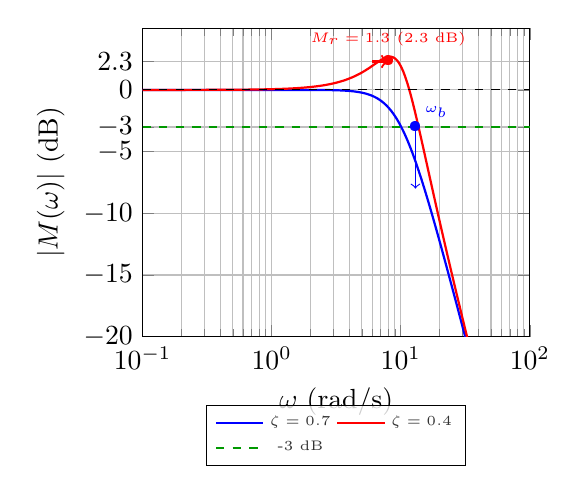
\begin{tikzpicture}
\begin{axis}[
    width=6.5cm, height=5.5cm,
    xmode=log,
    grid=both,
    xlabel={$\omega$ (rad/s)},
    ylabel={$|M(\omega)|$ (dB)},
    xmin=0.1, xmax=100,
    ymin=-20, ymax=5,
    ytick={-20,-15,-10,-5,-3,0,2.3},
    legend style={at={(0.5,-0.22)}, anchor=north, font=\tiny, 
                  fill=white, fill opacity=0.8, draw=black, 
                  legend columns=2},
]
% 典型闭环频率响应(不同阻尼)
\addplot[blue, thick, samples=200, domain=0.1:100] 
    {-20*log10(sqrt((1-(x/10)^2)^2 + (2*0.7*x/10)^2))};
\addlegendentry{$\zeta=0.7$}

\addplot[red, thick, samples=200, domain=0.1:100] 
    {-20*log10(sqrt((1-(x/10)^2)^2 + (2*0.4*x/10)^2))};
\addlegendentry{$\zeta=0.4$}

% -3dB线
\addplot[green!60!black, dashed, thick] coordinates {(0.1,-3) (100,-3)};
\addlegendentry{-3 dB}

% 0dB线
\addplot[black, dashed] coordinates {(0.1,0) (100,0)};

% 标注
\node[blue] at (axis cs:13,-3) {\textbullet};
\node[blue, above right] at (axis cs:13,-3) {\tiny $\omega_b$};
\draw[->, blue] (axis cs:13,-3) -- (axis cs:13,-8);

\node[red] at (axis cs:8,2.3) {\textbullet};
\node[red, above] at (axis cs:8,2.8) {\tiny $M_r = 1.3$ (2.3 dB)};
\draw[->, red, thick] (axis cs:6,2.3) -- (axis cs:8,2.3);

\end{axis}
\end{tikzpicture}
\end{center}

\small\textit{闭环幅频特性示例($\omega_n = 10$ rad/s)}

\vspace{0.3cm}
\textbf{4. 低频增益与稳态精度}

低频段幅值反映系统的稳态性能:

\begin{itemize}
    \item \textbf{0 型系统}:低频增益有限,位置误差有限
    \item \textbf{I 型系统}:低频段斜率 $-20$ dB/dec,位置误差为 0
    \item \textbf{II 型系统}:低频段斜率 $-40$ dB/dec,速度误差为 0
\end{itemize}

\vspace{0.2cm}
\textbf{5. 中频段特性与稳定性}

\begin{itemize}
    \item \textbf{斜率 $-20$ dB/dec}:系统一般稳定
    \item \textbf{斜率 $-40$ dB/dec}:需检查相位裕度
    \item \textbf{斜率 $-60$ dB/dec}:通常不稳定
\end{itemize}

\textbf{理想中频段特性:}
\begin{itemize}
    \item 斜率:$-20$ dB/dec
    \item 跨度:1.5-2 个十倍频
    \item 剪切频率 $\omega_c$ 选择合适(满足带宽和稳定性要求)
\end{itemize}
\end{minipage}

\vspace{0.3cm}
\textbf{例题:根据开环伯德图估算闭环系统性能指标。}

已知单位反馈系统开环传递函数 $G(s) = \frac{100}{s(1+0.1s)}$,从伯德图估算闭环性能。

\textit{解:}

\textbf{1. 求剪切频率(开环)}

$L(\omega) = 40 - 20\lg\omega - 20\lg\sqrt{1+0.01\omega^2} = 0$

近似求解:$\omega_c \approx 10$ rad/s

\textbf{2. 估算带宽(闭环)}

$\omega_b \approx \omega_c = 10$ rad/s $\implies$ 上升时间 $t_r \approx \frac{1.8}{10} = 0.18$ s

\textbf{3. 计算相位裕度}

$\phi(\omega_c) = -90° - \arctan(1) = -135°$ $\implies$ PM $= 45°$

\textbf{4. 估算超调量}

由 PM $= 45°$ 查表或用公式:$\sigma\% \approx 20\%$

等效阻尼比:$\zeta \approx 0.45$

\textbf{5. 估算谐振峰值}

$M_r \approx \frac{1}{2\zeta\sqrt{1-\zeta^2}} = \frac{1}{2 \times 0.45 \times 0.89} \approx 1.25$ $\implies$ 1.9 dB

\textbf{结论:}$\omega_b = 10$ rad/s,$t_r \approx 0.18$ s,$\sigma\% \approx 20\%$,$M_r \approx 1.25$(性能良好)

